%LaTeX template : http://systbio.org/files/SB_LaTeX_Template_txt_extension.txt
%Author instructions: http://www.oxfordjournals.org/our_journals/sysbio/for_authors/ms_preparation.html

\documentclass[12pt,letterpaper]{article}
\usepackage{natbib}

%Packages
\usepackage{pdflscape}
\usepackage{fixltx2e}
\usepackage{textcomp}
\usepackage{fullpage}
\usepackage{float}
\usepackage{latexsym}
\usepackage{url}
\usepackage{epsfig}
\usepackage{graphicx}
\usepackage{amssymb}
\usepackage{amsmath}
\usepackage{bm}
\usepackage{array}
\usepackage[version=3]{mhchem}
\usepackage{ifthen}
\usepackage{caption}
\usepackage{hyperref}
\usepackage{amsthm}
\usepackage{amstext}
\usepackage{enumerate}
\usepackage[osf]{mathpazo}
\usepackage{dcolumn}
\usepackage{lineno}
\usepackage{dcolumn}
\newcolumntype{d}[1]{D{.}{.}{#1}}

\pagenumbering{arabic}


%Pagination style and stuff
\linespread{2}
\raggedright
\setlength{\parindent}{0.5in}
\setcounter{secnumdepth}{0} 
\renewcommand{\section}[1]{%
\bigskip
\begin{center}
\begin{Large}
\normalfont\scshape #1
\medskip
\end{Large}
\end{center}}
\renewcommand{\subsection}[1]{%
\bigskip
\begin{center}
\begin{large}
\normalfont\itshape #1
\end{large}
\end{center}}
\renewcommand{\subsubsection}[1]{%
\vspace{2ex}
\noindent
\textit{#1.}---}
\renewcommand{\tableofcontents}{}

\begin{document}

%Running head
\begin{flushright}
Version dated: \today
\end{flushright}
\bigskip
\noindent RH: No effect of the K-Pg event on mammal disparity.

\bigskip
\medskip
\begin{center}

\noindent{\Large \bf Mammalian morphological diversity does not increase in response to the Cretaceous-Paleogene mass extinction and the extinction of the (non-avian) dinosaurs.} 
\bigskip

\noindent {\normalsize \sc Thomas Guillerme$^1$$^,$$^2$$^*$, and Natalie Cooper$^1$$^,$$^2$$^,$$^3$}\\
\noindent {\small \it 
$^1$School of Natural Sciences, Trinity College Dublin, Dublin 2, Ireland.\\
$^2$Trinity Centre for Biodiversity Research, Trinity College Dublin, Dublin 2, Ireland.\\
$^3$Department of Life Sciences, Natural History Museum, Cromwell Road, London, SW7 5BD, UK.}\\
\end{center}
\medskip
\noindent{*\bf Corresponding author.} \textit{guillert@tcd.ie}\\  
\vspace{1in}


%Line numbering
\modulolinenumbers[1]
\linenumbers

\renewcommand\thefigure{S\arabic{figure}}
\renewcommand\thetable{S\arabic{table}}

\section{Supplementary Information}

\subsection{Phylogenies}
This section (Figures S1 and S2) contains the trimmed phylogenies used in the analysis (see methods section in the main text for details).
% TG: this strap package is pure coded sweetness... I love these phylogenies!
\begin{figure}[!htbp]
\centering
    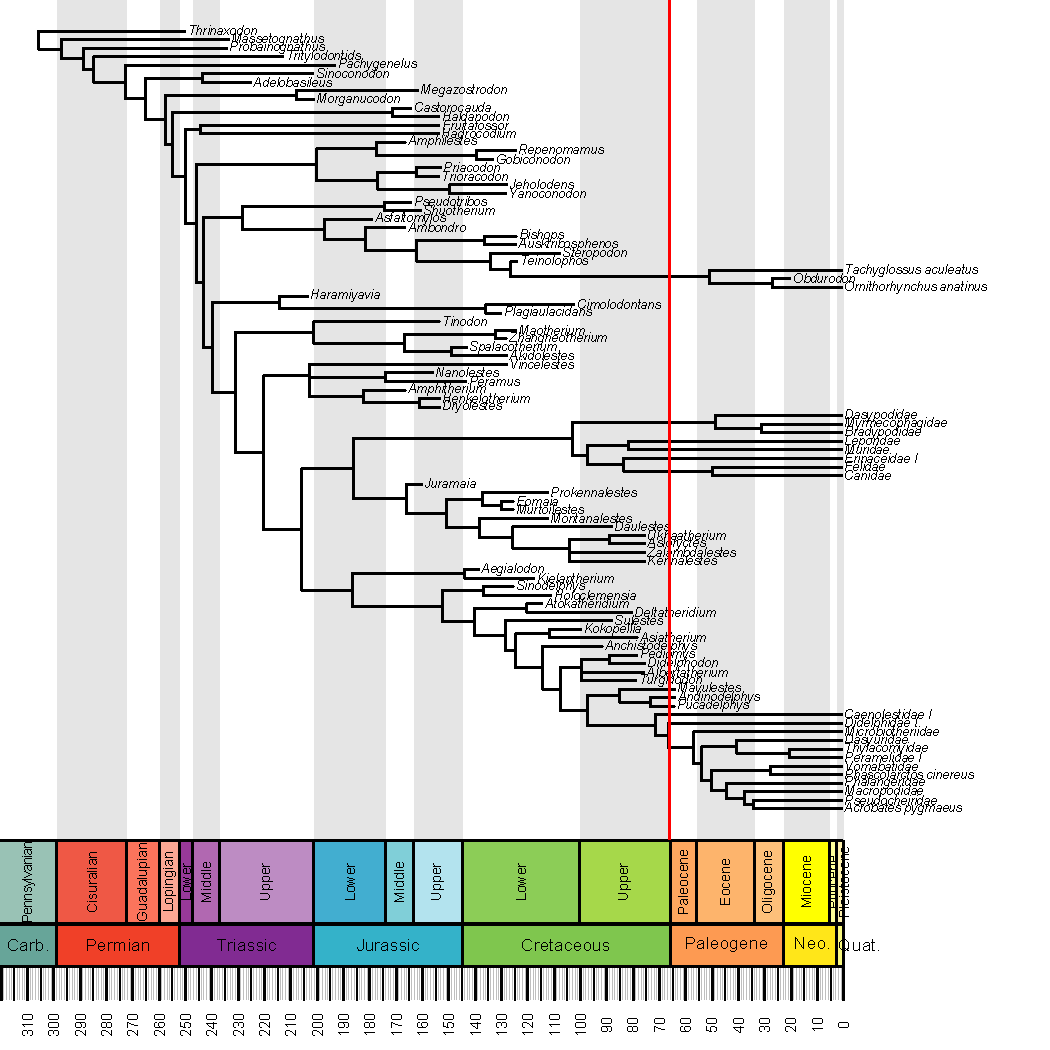
\includegraphics[keepaspectratio=true]{Figures/Figure_S1.pdf}
\caption{\textbf{Mammaliaformes phylogeny}. The phylogeny only contains taxa with overlapping cladistic data. The vertical red line represents the K-Pg boundary.}
\end{figure}

\begin{figure}[!htbp]
\centering
    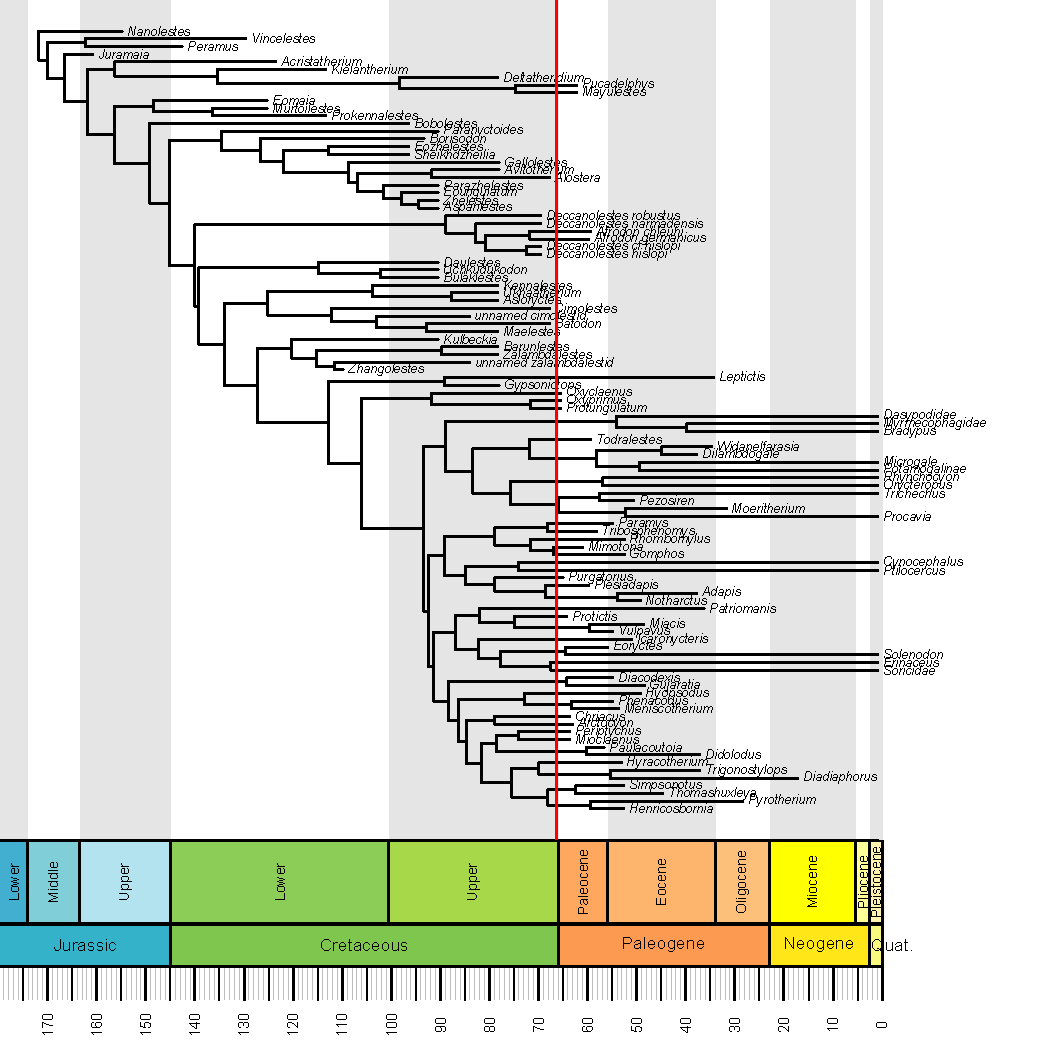
\includegraphics[keepaspectratio=true]{Figures/Figure_S2.pdf}
\caption{\textbf{Eutheria phylogeny}. The phylogeny only contains taxa with overlapping cladistic data. The vertical red line represents the K-Pg boundary.}
\end{figure}

\subsection{Rarefied analysis}
This section (Figures S3 to S5 and Table S1) contains the results from the rarefied Mammaliaformes and Eutheria datasets (see methods section in the main text for details).

\begin{figure}[!h]
\centering
    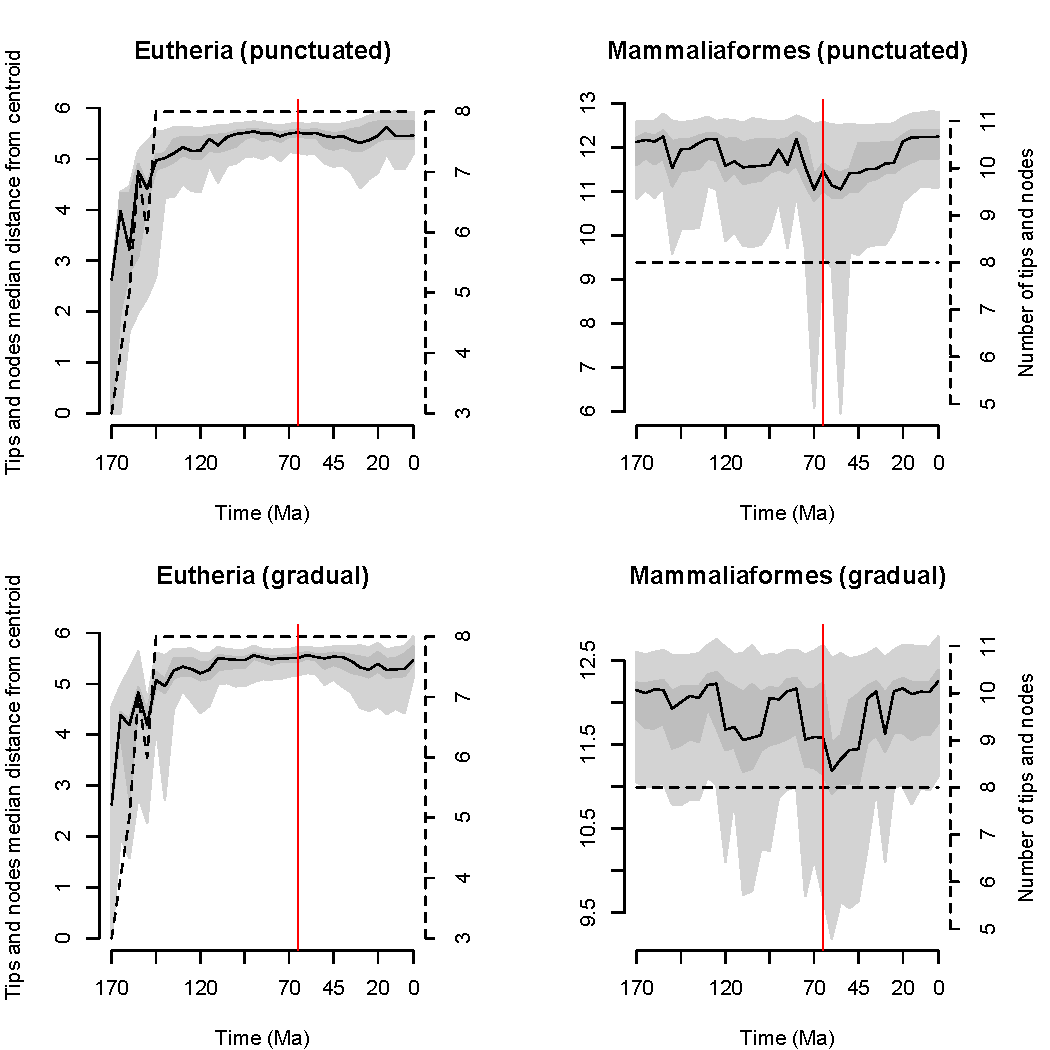
\includegraphics[keepaspectratio=true]{Figures/Figure_S3.pdf}
\caption{\scriptsize{Rarefied disparity through time in Eutheria and Mammaliaformes calculated using a model of punctuated (upper panels) or gradual (lower panels) evolution. The x axis represents time in millions of years before the present (Ma). The y axis represents disparity, measured as the median distance between the centroid of the ordinated space and the tips/nodes in each time subsample. The solid black lines show the mean disparity estimated from 1000 bootstrapped pseudoreplicates and confidence intervals (CI) are represented by the grey polygons (50\% CI in dark grey and 95\% CI in light grey). The dashed line and the right hand axis represents the number of tips/nodes in each time slice. The red vertical line indicates the Cretaceous-Paleogene (K-Pg) boundary (66 Ma). Note that scale bars differ among panels.}}
\label{fig:Fig_Rar_results}
\end{figure}


\begin{table}[ht]
\caption{\scriptsize{Results of rarefied t-tests comparing disparity at the last subsample of the Cretaceous (70 Ma) to subsamples of the Paleocene and Eocene, under both gradual and punctuated evolutionary models, in Mammaliaformes and Eutheria. Difference = mean difference in disparity between the two subsamples being compared; df = degrees of freedom; p value = original p value prior to Bonferonni correction.}}
\label{tab:Tab_beck}
\centering
\begin{tabular}{c|cccc|cccc}
  \hline
  \textbf{Subsamples} & \multicolumn{4}{c|}{\textbf{Gradual evolution model}} & \multicolumn{4}{c}{\textbf{Punctuated evolution model}} \\
  \textbf{compared} & \textbf{difference} & \textbf{df} & \textbf{t} & \textbf{p value} & \textbf{difference} & \textbf{df} & \textbf{t} & \textbf{p value} \\ 
  \hline
  \multicolumn{9}{c}{\textbf{Mammaliaformes}}\\
  \hline
  70 \textit{vs.} 65 & -0.360 & 21 & -0.486 & 0.632 & 0.040 & 21 & 0.054 & 0.957 \\ 
  70 \textit{vs.} 60 & -0.080 & 18 & -0.099 & 0.922 & 0.060 & 18 & 0.094 & 0.927 \\ 
  70 \textit{vs.} 55 & -0.090 & 19 & -0.110 & 0.914 & 0.050 & 19 & 0.082 & 0.936 \\ 
  70 \textit{vs.} 50 & -0.270 & 20 & -0.368 & 0.717 & 0.030 & 20 & 0.041 & 0.968 \\ 
  70 \textit{vs.} 45 & -0.310 & 23 & -0.419 & 0.679 & 0.200 & 23 & 0.285 & 0.778 \\ 
  70 \textit{vs.} 40 & -0.460 & 24 & -0.680 & 0.503 & -0.240 & 24 & -0.422 & 0.677 \\ 
  70 \textit{vs.} 35 & -0.510 & 26 & -0.742 & 0.465 & -0.100 & 26 & -0.159 & 0.875 \\ 
  \hline
  \multicolumn{9}{c}{\textbf{Eutheria}}\\
  \hline
  70 \textit{vs.} 65 & -0.020 & 84 & -0.139 & 0.890 & 0.020 & 84 & 0.101 & 0.920 \\ 
  70 \textit{vs.} 60 & 0.020 & 76 & 0.095 & 0.925 & 0.070 & 76 & 0.386 & 0.701 \\ 
  70 \textit{vs.} 55 & 0.010 & 75 & 0.076 & 0.940 & 0.020 & 75 & 0.111 & 0.912 \\ 
  70 \textit{vs.} 50 & 0.090 & 68 & 0.453 & 0.652 & 0.040 & 68 & 0.232 & 0.817 \\ 
  70 \textit{vs.} 45 & 0.120 & 64 & 0.563 & 0.575 & 0.110 & 64 & 0.562 & 0.576 \\ 
  70 \textit{vs.} 40 & 0.100 & 64 & 0.473 & 0.638 & 0.070 & 64 & 0.383 & 0.703 \\ 
  70 \textit{vs.} 35 & 0.120 & 60 & 0.515 & 0.608 & 0.040 & 60 & 0.195 & 0.846 \\ 
   \hline
\end{tabular}
\end{table}

\begin{figure}[!h]
\centering
    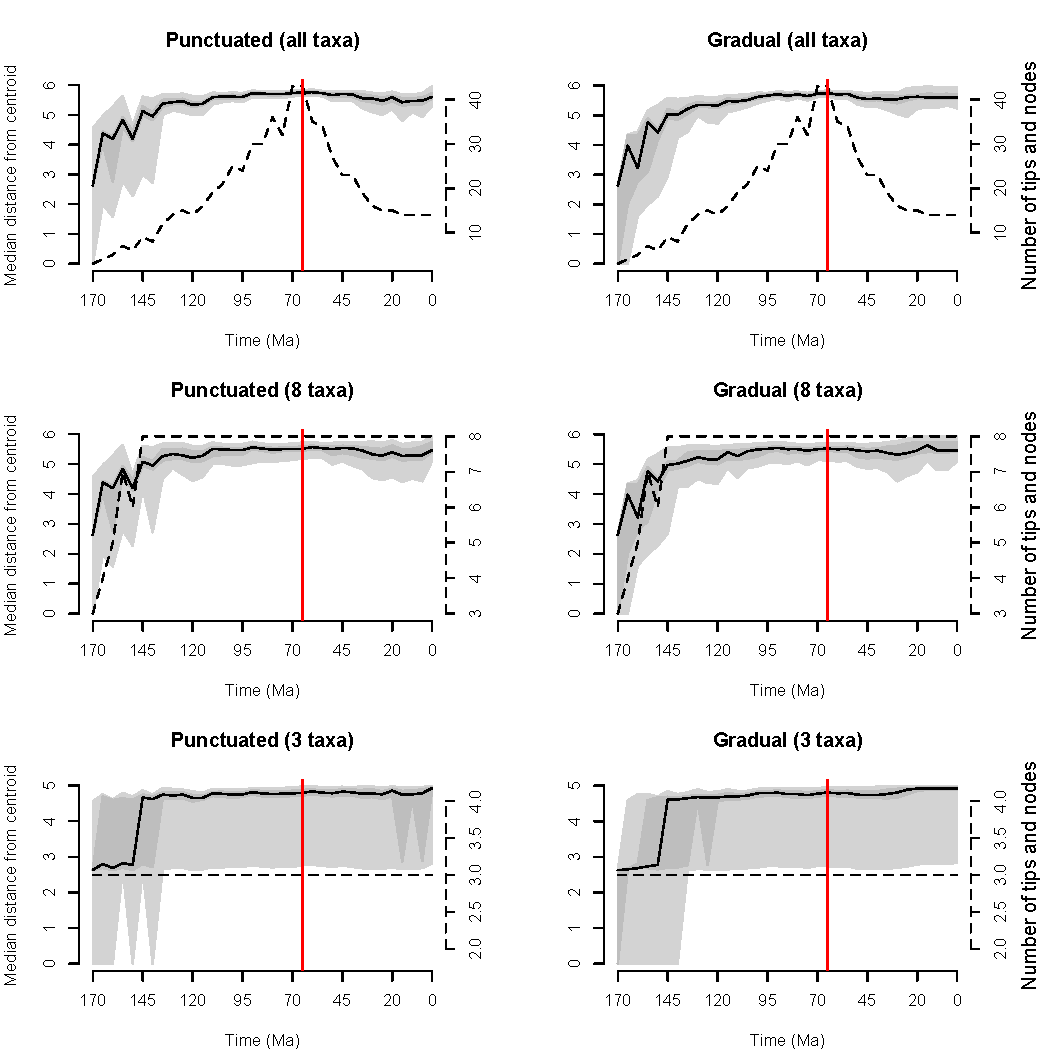
\includegraphics[keepaspectratio=true]{Figures/Figure_S4.pdf}
\caption{\scriptsize{Variations of disparity through time among Eutheria with a punctuated or gradual evolution model for different number of taxa (rarefaction). The x axis represents the time in Million of years ago (Mya). The y axis represents the disparity measured as the median distance from centroid per sub-sample. The solid black lines is the mean disparity; the confidence intervals (CI) are represent by the grey polygons (50\% CI in dark grey and 95\% CI in light grey). The dashed line represent the species richness in each sub-sample (values are reported on the right hand side of each graphs). The red vertical line represents the K-Pg boundary (66 Mya).}}
\end{figure}

\begin{figure}[!h]
\centering
    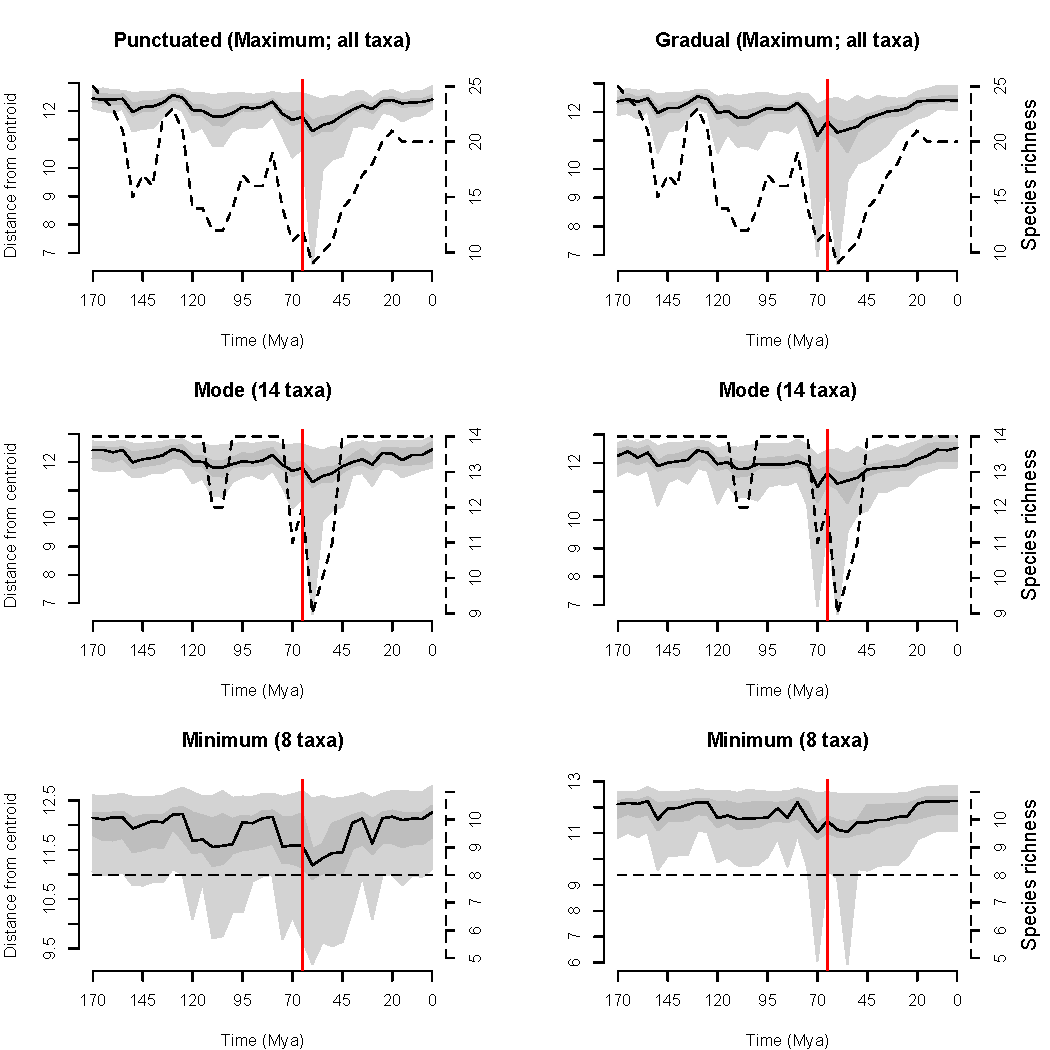
\includegraphics[keepaspectratio=true]{Figures/Figure_S5.pdf}
\caption{\scriptsize{Observed and rarefied variation of disparity through time among Mammaliaformes with a punctuated or gradual evolution model. The x axis represents the time in Million of years ago (Mya). The y axis represents the disparity measured as the median distance from centroid per sub-sample. The solid black lines is the mean disparity; the confidence intervals (CI) are represent by the grey polygons (50\% CI in dark grey and 95\% CI in light grey). The dashed line represent the species richness in each sub-sample (values are reported on the right hand side of each graphs). The red vertical line represents the K-Pg boundary (66 Mya).}}
\end{figure}


\subsection{Comparison of different disparity metrics and time sampling methods}
This section (Figure S6, S7, S8 and S9) contains the results of the variation of disparity through time analyses for Mammaliaformes and Eutheria using all the disparity metrics and methods for sampling disparity through time.
The different disparity metrics are the median distance from centroid (see main text for details), and the sum and products of ranges and variances of the cladisto-space dimensions.
The sum and products of ranges and variances are calculated as follows:

\begin{equation}
    \text{Sum of ranges}=\sum{(max(\mathbf{v}_{n})-min(\mathbf{v}_{n}))}
\end{equation}
\begin{equation}
    \text{Sum of variances}=\sum{(\sigma^{2}(\mathbf{v}_{n}))}
\end{equation}
\begin{equation}
    \text{Product of ranges}=\prod{(max(\mathbf{v}_{n})-min(\mathbf{v}_{n}))}
\end{equation}
\begin{equation}
    \text{Product of variances}=\prod{(\sigma^{2}(\mathbf{v}_{n}))}
\end{equation}

\noindent
where $\mathbf{v}_{n}$ is any of the $n$ eigenvectors (i.e. any of the $n$ dimensions of the cladisto-space), $max$ and $min$ are respectively the maximum and minimum values of each eigenvector $\mathbf{v}_{n}$, and $\sigma^{2}$ is the variance of each eigenvector $\mathbf{v}_{n}$. 

The different time sampling methods are as follows:
\begin{enumerate}
\item \textbf{Intervals (tips only)}.
We selected every tip present at every geological stage (i.e. the smaller stratigraphic units) from the early Middle Jurassic (Bajocian, starting at 170.3 Ma) to the present.
We collapsed together every stage containing fewer than three tips so that every time interval contained at least three tips.
Note that some tips were present in multiple stages due to their occurrence data (see main text for details).
\item \textbf{Intervals (tips and nodes)}.
We selected tips and nodes present at every stage from the early Middle Jurassic (Bajocian, starting at 170.3 Ma) to the present.
We collapsed together every stage containing fewer than three elements (tips and/or nodes).
\item \textbf{Slices (punctuated)}.
These are the results presented in the main text where the cladisto-space is sampled every 5 Ma and the mode of evolution between each subsample is assumed to be punctuated (randomly selecting either data from the descendant or the ancestor when slicing through a branch; see main text for details).
\item \textbf{Slices (punctuated: ACCTRAN)}.
Similar to the slices (punctuated) method but data are always selected from the descendant (see main text for details).
\item \textbf{Slices (punctuated: DELTRAN)}.
Similar to the slices (punctuated) method but data are always selected from the ancestor (see main text for details).
\item \textbf{Slices (gradual)}.
These are the results presented in the main text where the cladisto-space is sampled every 5 Ma and the mode of evolution is assumed to be gradual (data is selected from the descendant or the ancestor based on branch length; see main text for details).
\end{enumerate}
We also rarefied both datasets for all the metrics and all the methods using the minimum of three taxa for the interval methods, and eight taxa for the slices methods.

\begin{landscape}
\begin{figure}[!htbp]
\centering
    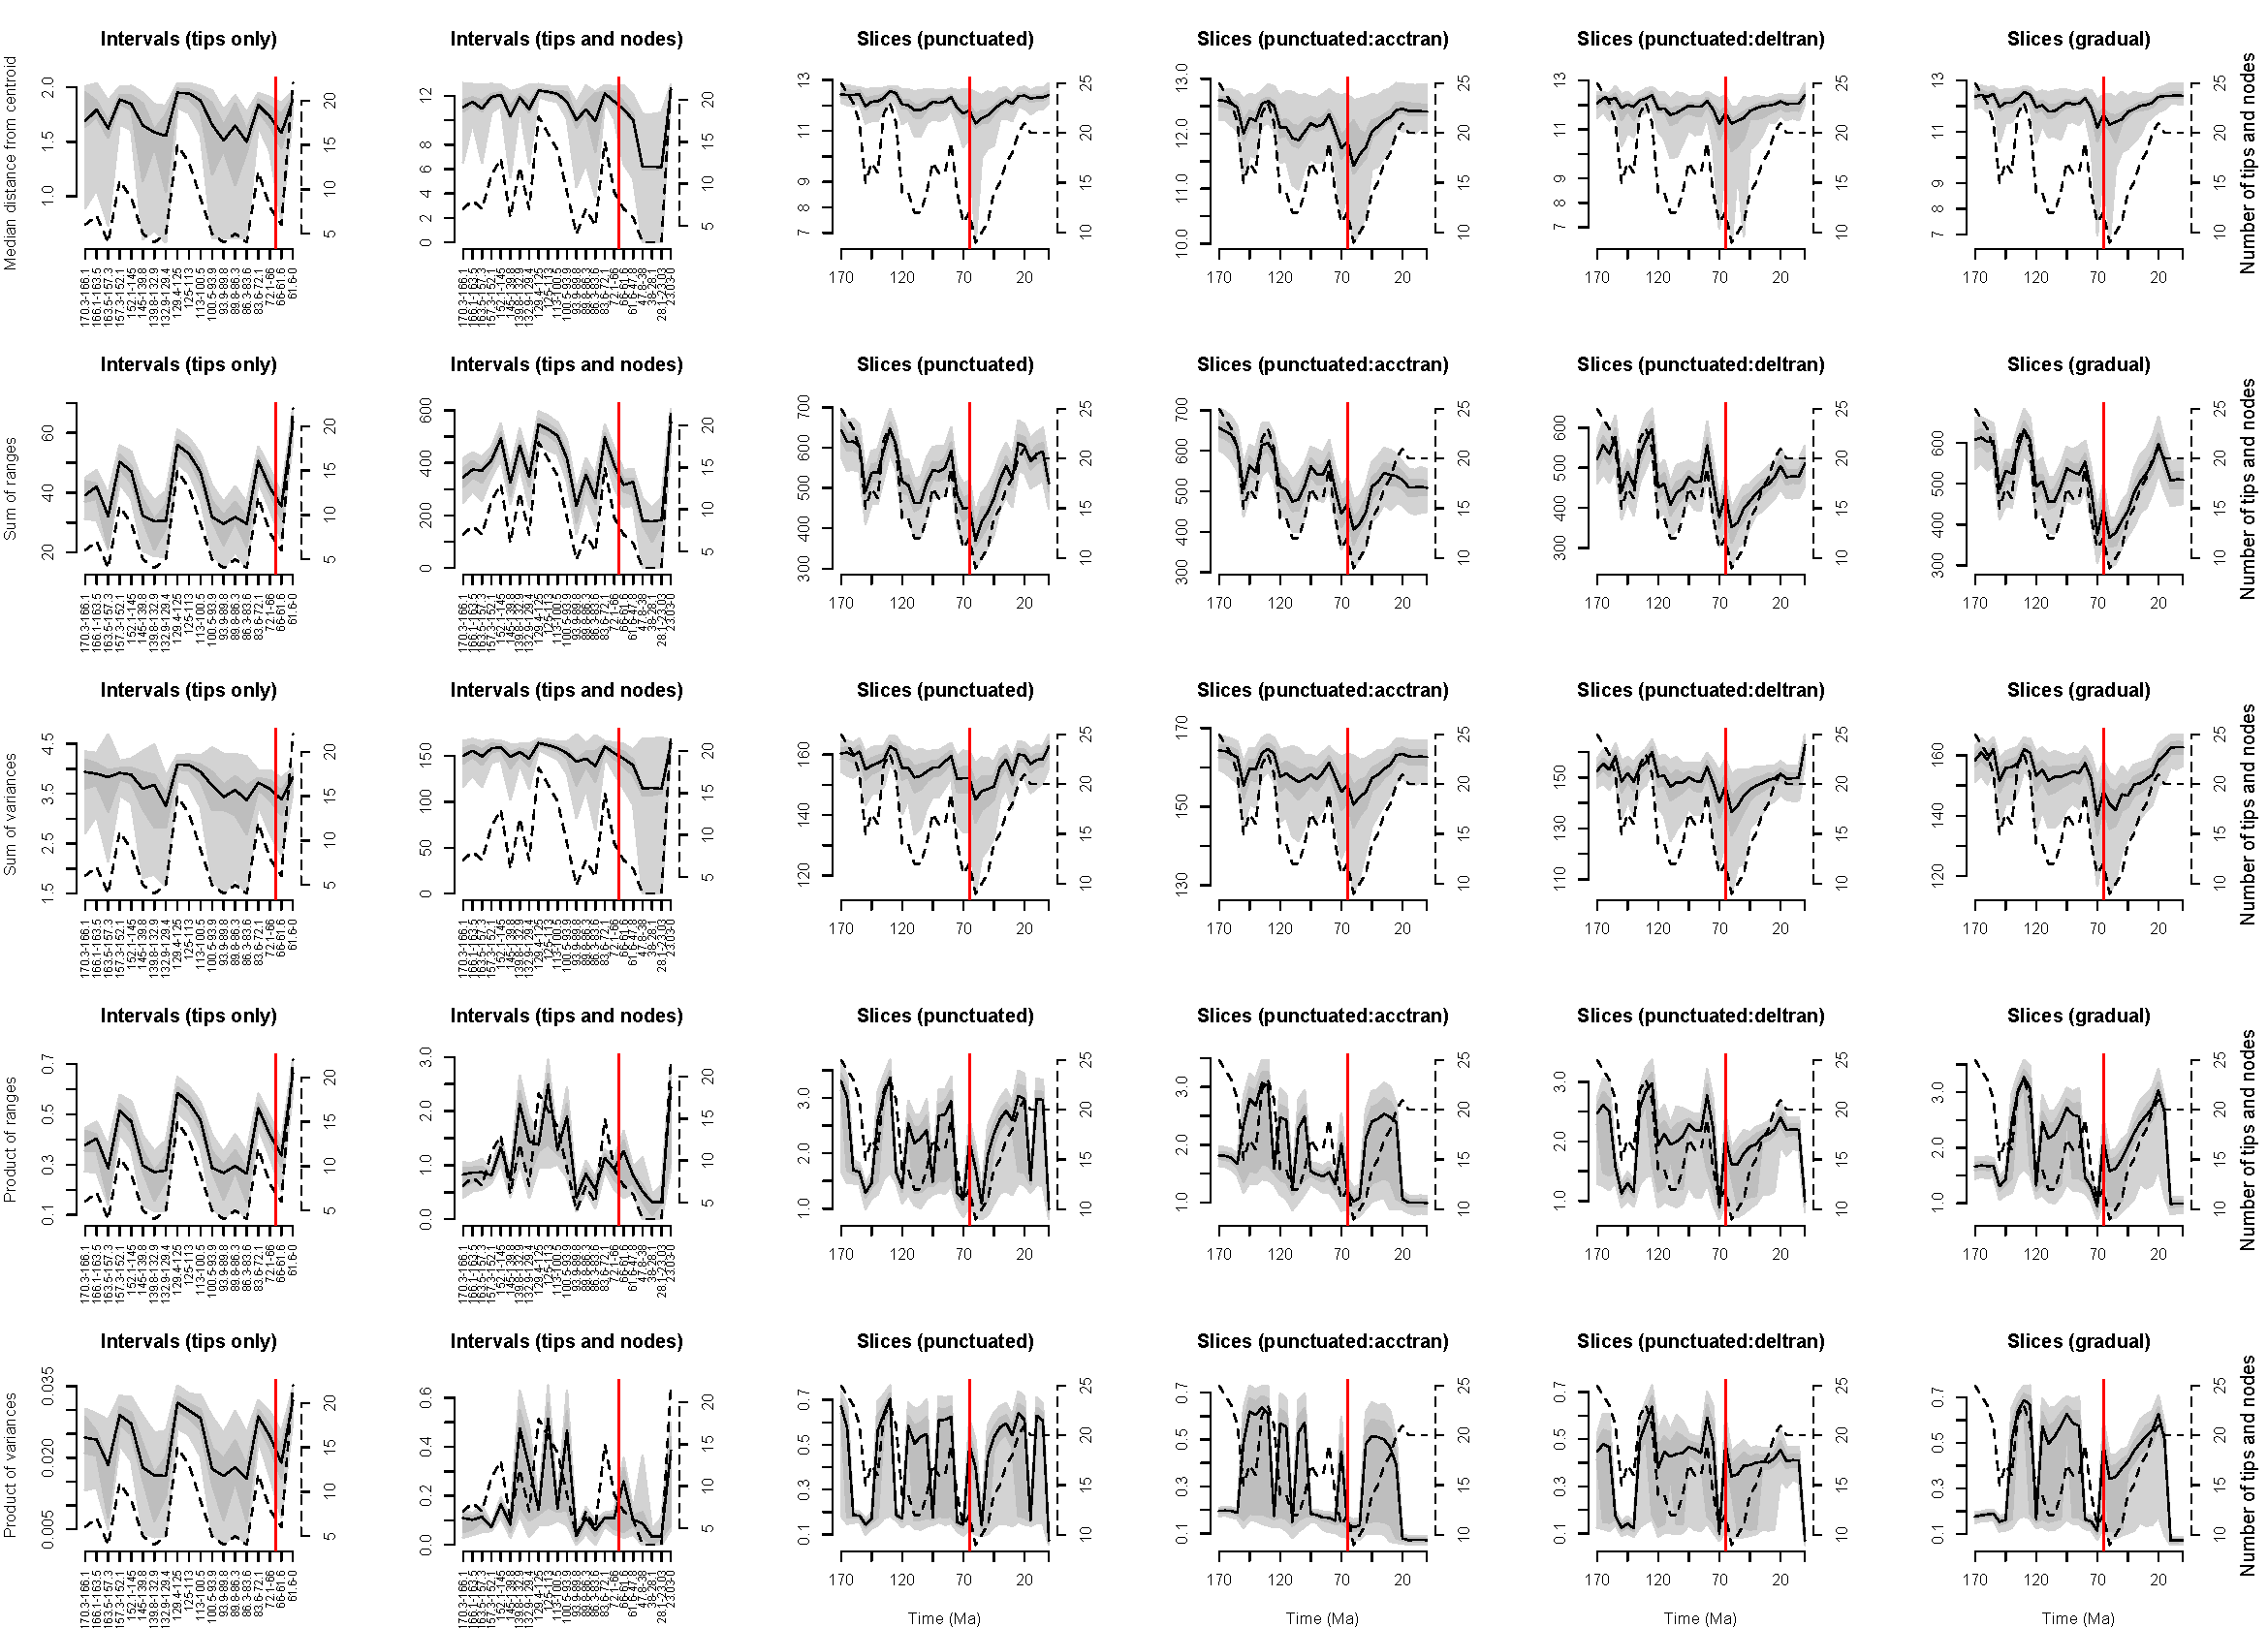
\includegraphics[width=\textwidth,height=\textheight,keepaspectratio]{Figures/Figure_S6.pdf}
\caption{\scriptsize{Variations of disparity through time among Mammaliaformes with disparity measurements and methods for sampling disparity through time. The x axis represents the time in Million of years ago (Mya). The y axis represents the disparity measured as the median distance from centroid per sub-sample. The solid black lines is the mean disparity; the confidence intervals (CI) are represent by the grey polygons (50\% CI in dark grey and 95\% CI in light grey). The dashed line represent the species richness in each sub-sample (values are reported on the right hand side of each graphs). The red vertical line represents the K-Pg boundary (66 Mya).}}
\end{figure}
\end{landscape}

\begin{landscape}
\begin{figure}[!htbp]
\centering
    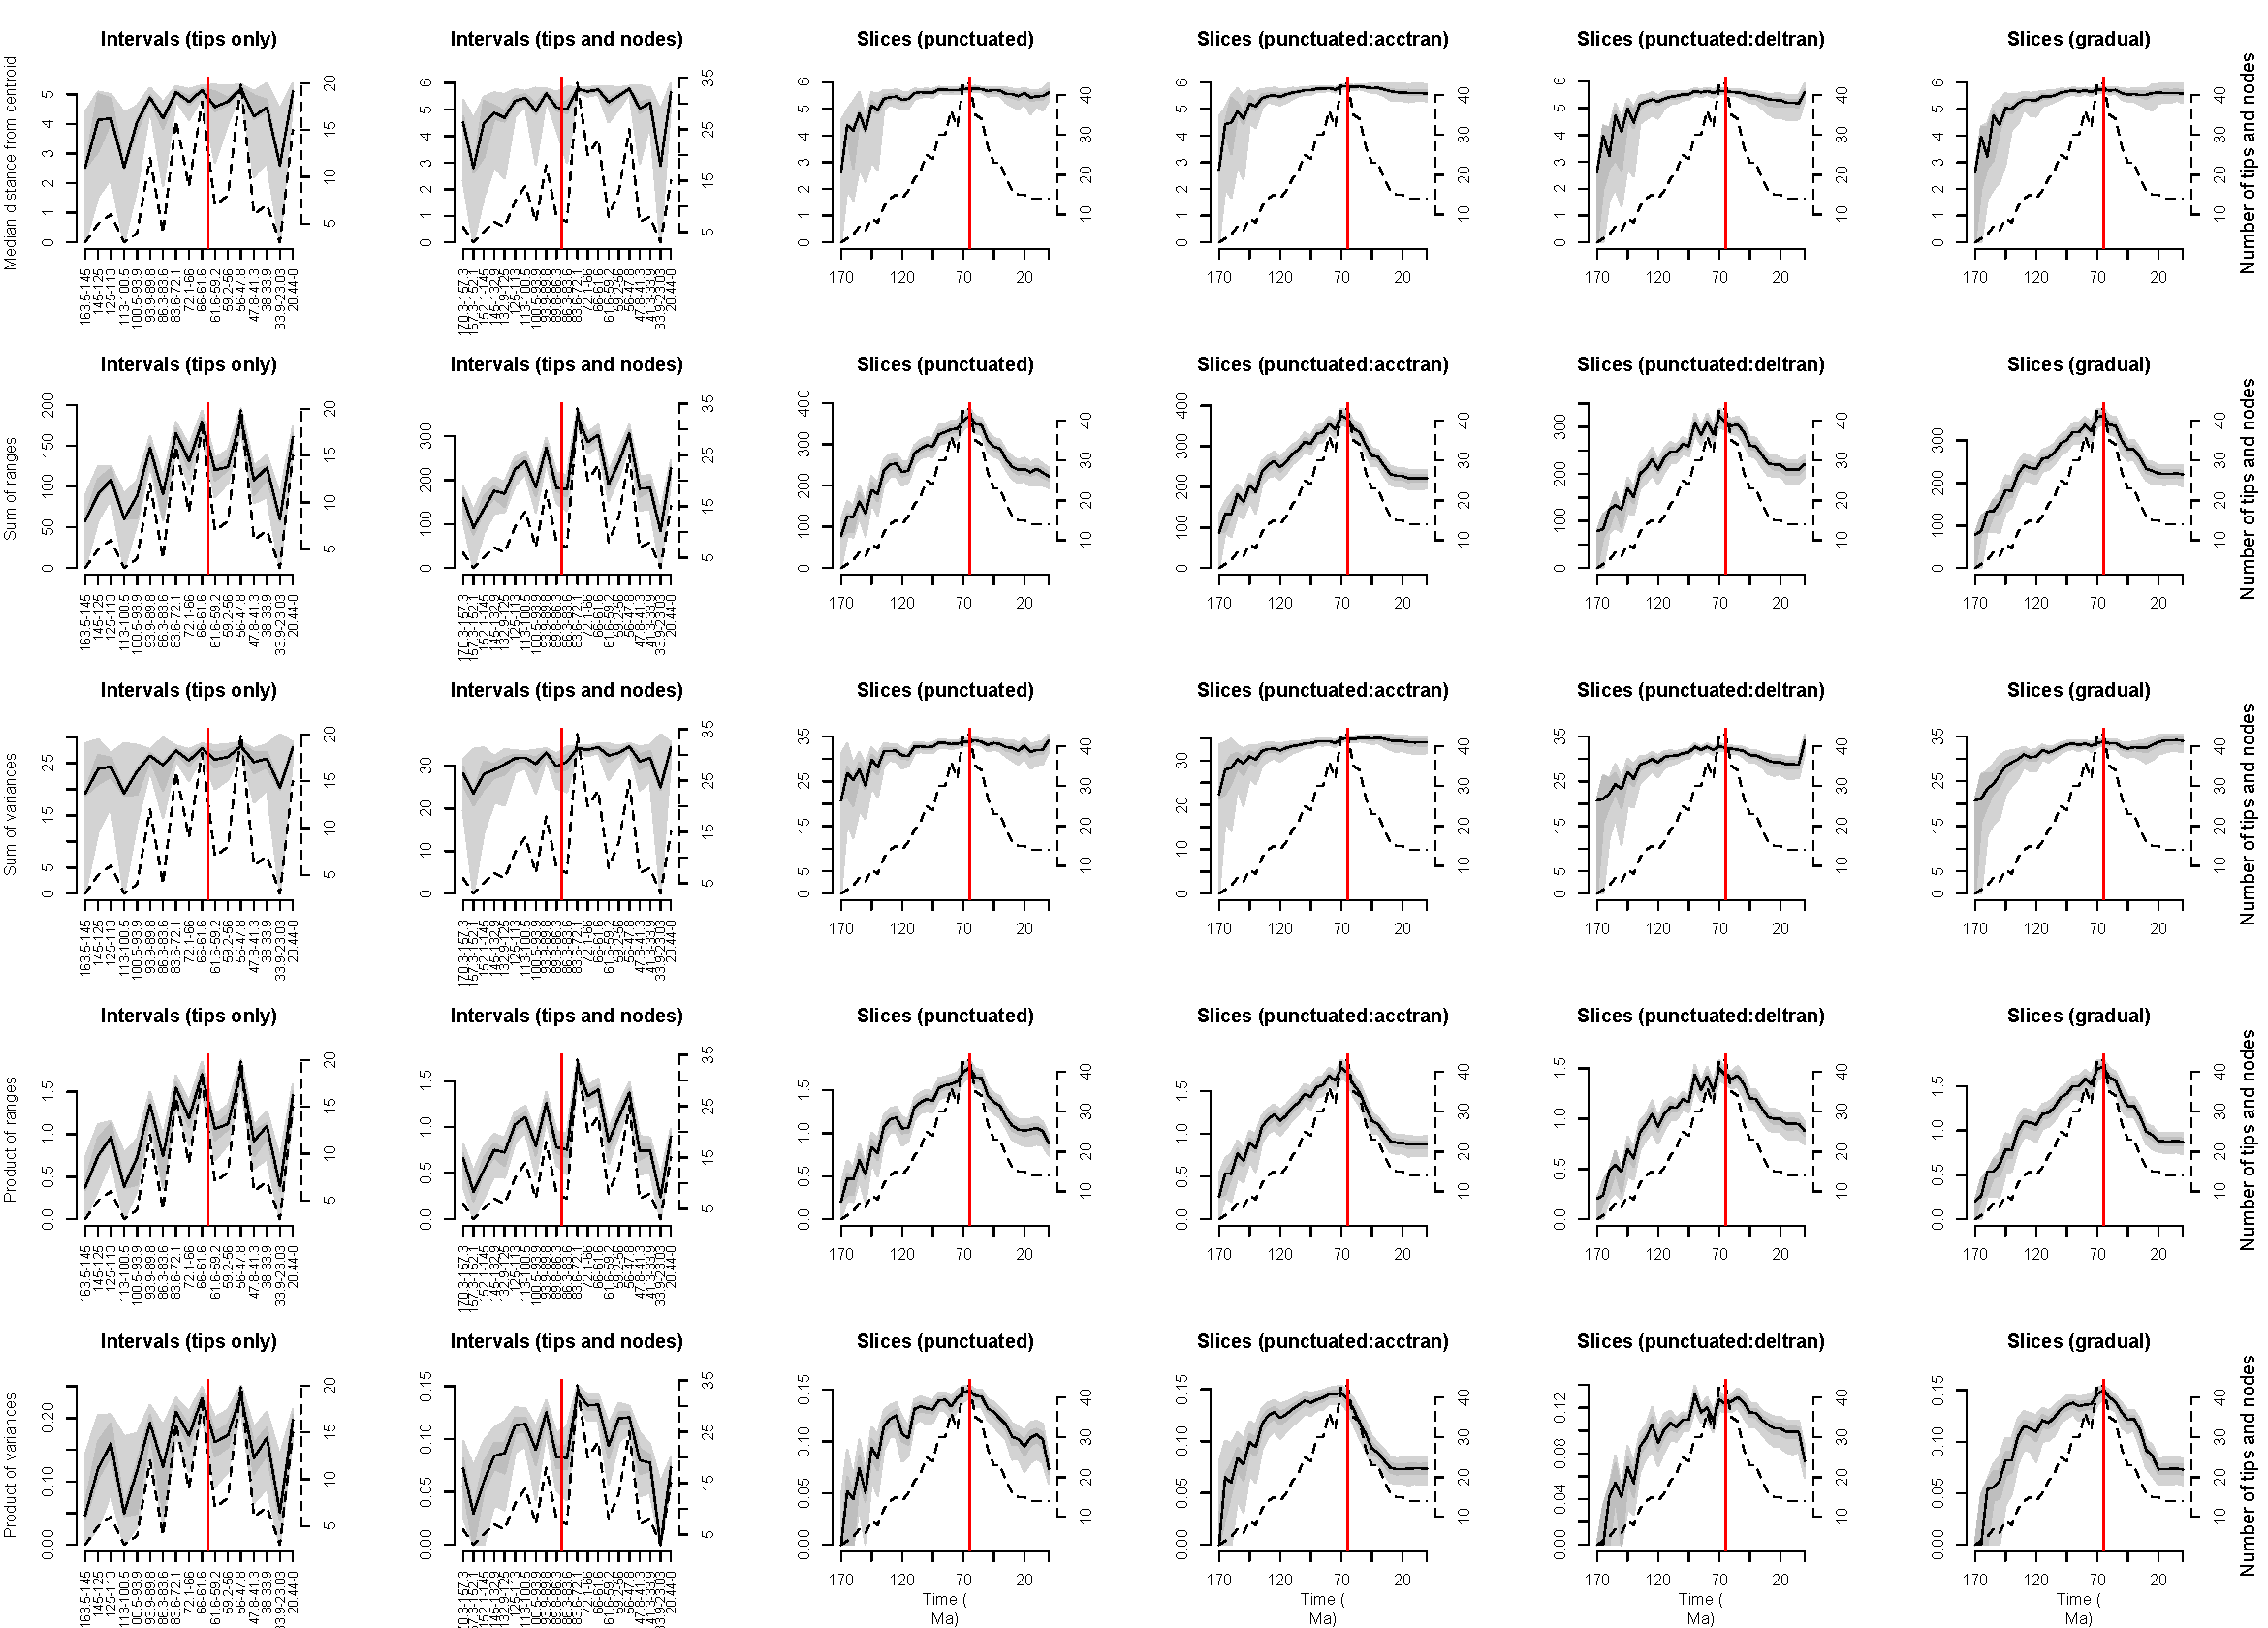
\includegraphics[width=\textwidth,height=\textheight,keepaspectratio]{Figures/Figure_S7.pdf}
\caption{\scriptsize{Variations of disparity through time among Eutheria with disparity measurements and methods for sampling disparity through time. The x axis represents the time in Million of years ago (Mya). The y axis represents the disparity measured as the median distance from centroid per sub-sample. The solid black lines is the mean disparity; the confidence intervals (CI) are represent by the grey polygons (50\% CI in dark grey and 95\% CI in light grey). The dashed line represent the species richness in each sub-sample (values are reported on the right hand side of each graphs). The red vertical line represents the K-Pg boundary (66 Mya).}}
\end{figure}
\end{landscape}

\begin{landscape}
\begin{figure}[!htbp]
\centering
    \includegraphics[width=\textwidth,height=\textheight,keepaspectratio]{Figures/Figure_S8.pdf}
\caption{\scriptsize{Variations of disparity through time among Mammaliaformes with disparity measurements and methods for sampling disparity through time (rarefied with 3 taxa for the interval method and 8 taxa for the slice method). The x axis represents the time in Million of years ago (Mya). The y axis represents the disparity measured as the median distance from centroid per sub-sample. The solid black lines is the mean disparity; the confidence intervals (CI) are represent by the grey polygons (50\% CI in dark grey and 95\% CI in light grey). The dashed line represent the species richness in each sub-sample (values are reported on the right hand side of each graphs). The red vertical line represents the K-Pg boundary (66 Mya).}}
\end{figure}
\end{landscape}

\begin{landscape}
\begin{figure}[!htbp]
\centering
    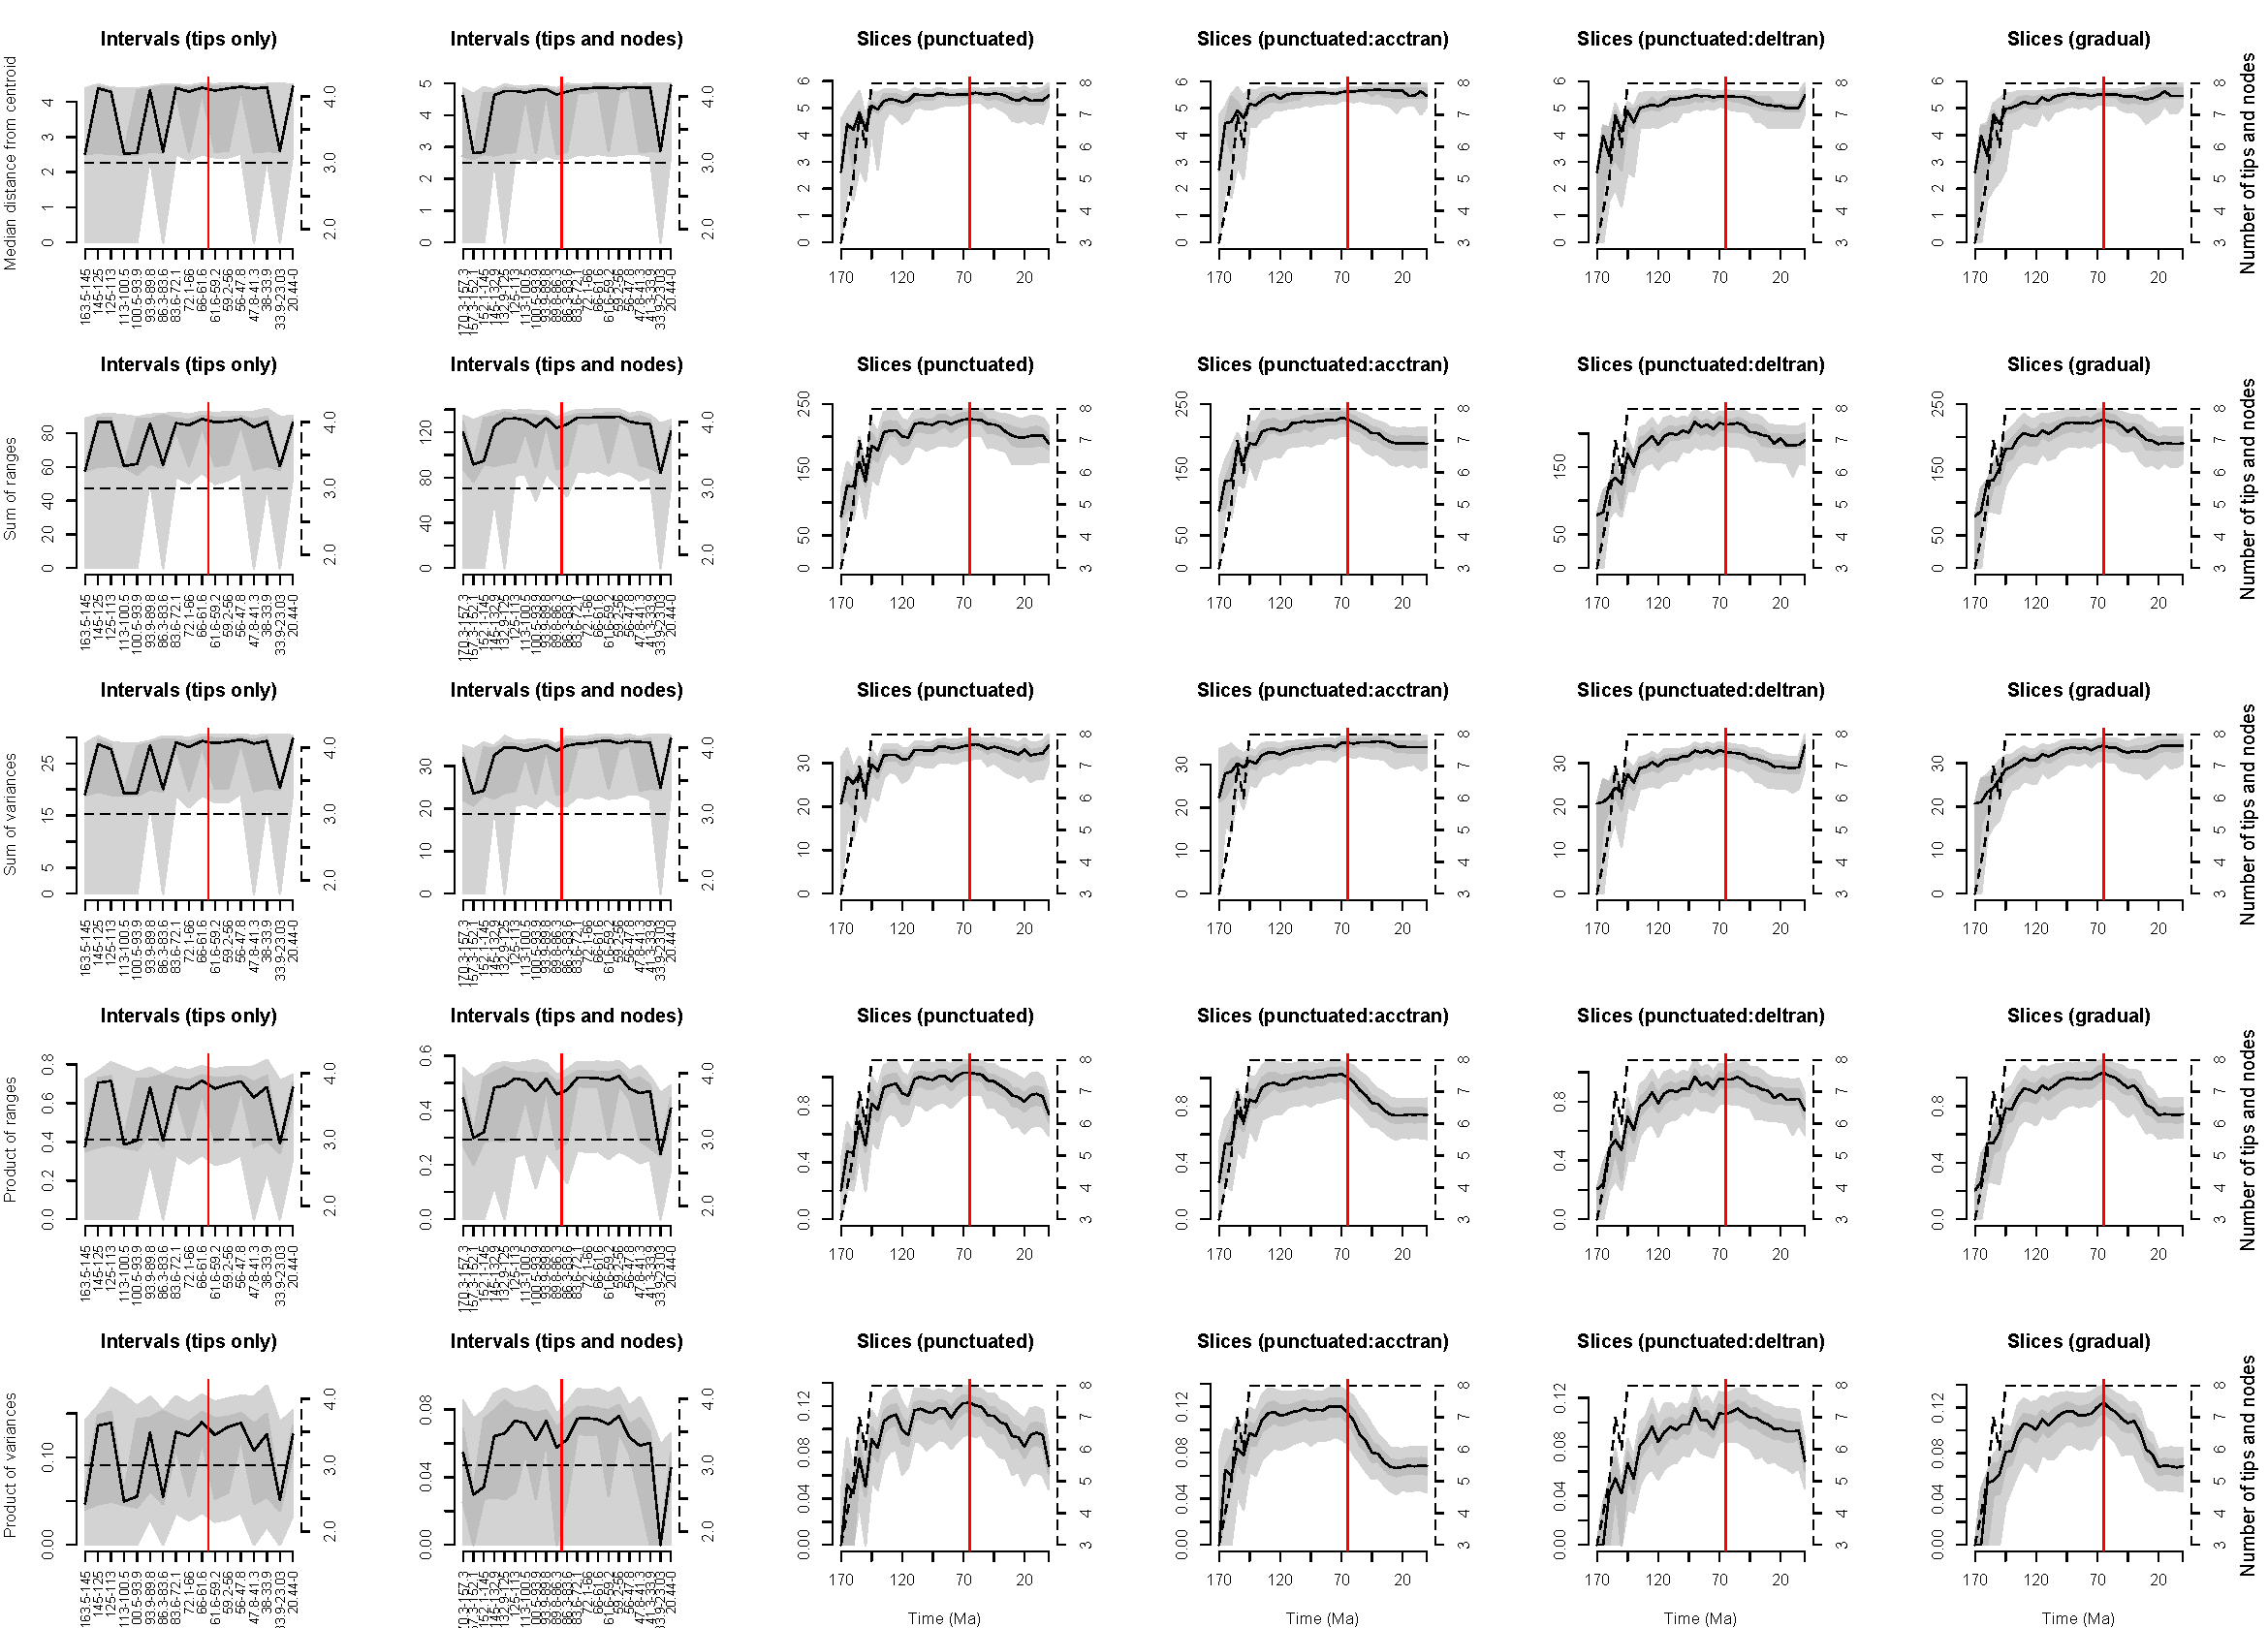
\includegraphics[width=\textwidth,height=\textheight,keepaspectratio]{Figures/Figure_S9.pdf}
\caption{\scriptsize{Variations of disparity through time among Eutheria with disparity measurements and methods for sampling disparity through time (rarefied with 3 taxa for the interval method and 8 taxa for the slice method). The x axis represents the time in Million of years ago (Mya). The y axis represents the disparity measured as the median distance from centroid per sub-sample. The solid black lines is the mean disparity; the confidence intervals (CI) are represent by the grey polygons (50\% CI in dark grey and 95\% CI in light grey). The dashed line represent the species richness in each sub-sample (values are reported on the right hand side of each graphs). The red vertical line represents the K-Pg boundary (66 Mya).}}
\end{figure}
\end{landscape}


\end{document}